\documentclass[acmsmall,review,anonymous]{acmart}

%\settopmatter{printfolios=true,printccs=false,printacmref=false}

\overfullrule=1mm
\citestyle{acmauthoryear}
%\setcitestyle{round}

\usepackage{alltt}
\usepackage{amssymb}
\usepackage{calc}
\usepackage{cleveref}
\usepackage{listings}
\usepackage{mathpartir}
\usepackage{pifont}
\usepackage{tikz}
\usepackage{wrapfig}
\usepackage{xcolor}
\usetikzlibrary{shapes.geometric}

\begin{document}

\title{Millions of Type Errors}

\author{Ben Greenman}
\orcid{0000-0001-7078-9287}
\affiliation{%
  \institution{Brown University}
  \city{Providence}
  \state{Rhode Island}
  \country{USA}
}
\email{benjaminlgreenman@gmail.com}

\author{Alan Jeffrey}
\orcid{TODO}
\affiliation{%
  \institution{Roblox}
  \city{}
  \state{}
  \country{USA}
}
\email{}

\author{Mitesh Shah}
\orcid{TODO}
\affiliation{%
  \institution{Roblox}
  \city{}
  \state{}
  \country{USA}
}
\email{}

\author{Shriram Krishnamurthi}
\orcid{0000-0001-5184-1975}
\affiliation{%
  \institution{Brown University}
  \city{Providence}
  \state{Rhode Island}
  \country{USA}
}
\email{shriram@brown.edu}

%\renewcommand{\shortauthors}{...}

%%
%% The abstract is a short summary of the work to be presented in the
%% article.
\begin{abstract}
  TBD
\end{abstract}


%%
%% The code below is generated by the tool at http://dl.acm.org/ccs.cfm.
%% Please copy and paste the code instead of the example below.

\begin{CCSXML}
<ccs2012>
<concept>
<concept_id>10011007.10011006.10011039.10011311</concept_id>
<concept_desc>Software and its engineering~Semantics</concept_desc>
<concept_significance>500</concept_significance>
</concept>
<concept>
<concept_id>10011007.10011006.10011008.10011024.10011032</concept_id>
<concept_desc>Software and its engineering~Constraints</concept_desc>
<concept_significance>100</concept_significance>
</concept>
<concept>
<concept_id>10011007.10011006.10011008.10011009.10011012</concept_id>
<concept_desc>Software and its engineering~Functional languages</concept_desc>
<concept_significance>100</concept_significance>
</concept>
</ccs2012>
\end{CCSXML}

\ccsdesc[500]{Software and its engineering~Semantics}
\ccsdesc[100]{Software and its engineering~Constraints}
\ccsdesc[100]{Software and its engineering~Functional languages}

\keywords{types, gradual typing, telemetry, user study, large-scale study}

\maketitle

\section{Introduction}
\label{s:introduction}

millions of creators:
 gradual types,
 success types,
 semantic subtyping

millions (?) of telemetry records

takeaways about adoption,
 errors by mode (nocheck, nonstrict, strict),
 patterns of use,


\section{Roblox Contex}

\paragraph{Creating Experiences}

more than games

telemetry gets a session id per experience


\paragraph{Script, Module}

%% https://create.roblox.com/docs/education/coding-6/intro-to-module-scripts

script = code that runs, can have many scripts in a codebase

module = library, reusable functions, doesn't run directly

scripts are fine for basic games. professional developers are much more likely to use modules.


\paragraph{Data Model}

changes to DM can give huge type error changes

moving (re-parent) a node changes the type of the DM, unsoundness in type system

type checker assumes initial state


\section{Telemetry Design}

No PII whatsoever

Random session selection

Random events during session, except module switch.

No access to other key events: save, exit.
Don't want access to run, publish.

\url{https://docs.google.com/document/d/1DnKvw8x1jy0EWCbBSM8neKULWz7WAg1OauKy7qqYqkI/edit}


\section{Predictions}
%%bg: merge with prev section, on telemetry design?

nocheck forcestrict keep growing

nonstrict te tend to zero, fixing your program should fix the errors, no false positives

nonstrict fs unclear


\section{Results}
\label{s:data}

\begin{figure}[t]
  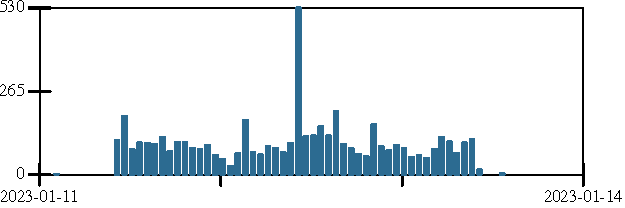
\includegraphics{img/row-distribution.pdf}
  \Description{TBD: histogram with about 100 records per hour except for a 600-record spike near the end of Jan 12th.}
  \caption{Telemetry records per hour. Each tick on the $x$-axis marks the start of a new day in California.}
  \label{f:records-per-hour}
\end{figure}

\Cref{f:records-per-hour} shows when data arrived across the whole dataset.


\section{Interpretation}

Error 1000 = type mismatch (subtyping etc);
1001 = unknown symbol;
\ldots

% https://github.com/Roblox/luau/blob/master/Analysis/include/Luau/Error.h


\begin{verbatim}
 require(foobar)
  foobar is a module script in the data model
 require(foo.bar.b)
  - could be edit in progress
  - could be renamed module
  - 
\end{verbatim}



\section{Related Work}
\label{s:related}

Mind your language~\cite{mfk-onward-2011}.


\section{Discussion}
\label{s:conclusion}
\label{s:discussion}



\begin{acks}
  TBD

Greenman was supported by
  \grantsponsor{NSF}{NSF}{https://www.nsf.gov} grant
 \href{"https://www.nsf.gov/awardsearch/showAward?AWD_ID=2030859"}{\grantnum{NSF}{CCF 2030859}}
  to the CRA for the \href{https://cifellows2020.org}{CIFellows} project.
\end{acks}

\bibliographystyle{ACM-Reference-Format}
\bibliography{bib}

\end{document}
\endinput
